% =============================================================================
%  Diagrama de flujo IDC multiobjetivo (IDC-MO), en español, vectorial.
%  Reemplaza a fig_idc_mo.jpg (inglés, con erratas). Compilar: pdflatex.
%  Sin babel: con [spanish] los caracteres > y % se vuelven activos y rompen
%  la sintaxis >= de TikZ y los % matemáticos.
% =============================================================================
\documentclass[border=6pt]{standalone}
\usepackage[T1]{fontenc}
\usepackage[utf8]{inputenc}
\usepackage{tikz}
\usetikzlibrary{positioning,shapes.geometric,arrows.meta,calc,backgrounds,fit}

\definecolor{idcblue}{RGB}{31,103,131}

\begin{document}
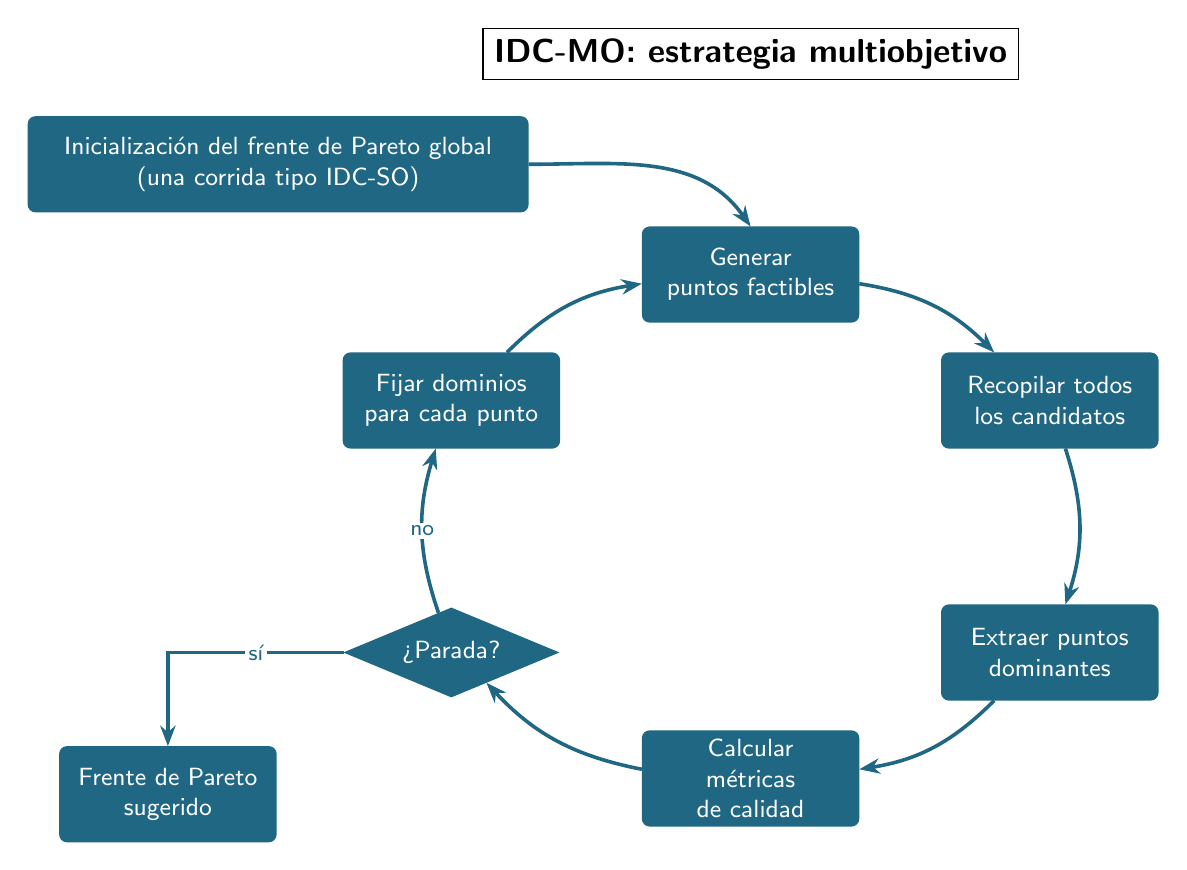
\begin{tikzpicture}[
  font=\sffamily\small,
  >={Stealth[length=3mm]},
  box/.style   = {rectangle, rounded corners=2.5pt, draw=idcblue, fill=idcblue,
                  text=white, align=center, minimum height=12mm, text width=26mm,
                  inner sep=2pt, line width=0.6pt},
  dec/.style   = {diamond, draw=idcblue, fill=idcblue, text=white, aspect=2.4,
                  align=center, inner sep=1pt, text width=18mm, minimum height=11mm},
  fl/.style    = {-{Stealth[length=2.6mm]}, idcblue, line width=1.3pt},
  lab/.style   = {font=\sffamily\footnotesize, fill=white, inner sep=1.2pt},
  title/.style = {draw=black, fill=white, rounded corners=0pt, font=\sffamily\bfseries\large,
                  inner sep=4pt}
]

% --- Título ------------------------------------------------------------------
\node[title] at (9.3,10.4) {IDC-MO: estrategia multiobjetivo};

% --- Inicialización (caja ancha, dos filas) ---------------------------------
\node[box, text width=62mm, minimum height=12mm] (init) at (3.3,9.0)
     {Inicialización del frente de Pareto global\\ (una corrida tipo IDC-SO)};

% --- Lazo circular (sentido horario, elipse centrada en (9.3,4.4)) ----------
\node[box] (gen)   at (9.3,7.6) {Generar\\ puntos factibles};
\node[box] (coll)  at (13.1,6.0) {Recopilar todos\\ los candidatos};
\node[box] (domi)  at (13.1,2.8) {Extraer puntos\\ dominantes};
\node[box] (metr)  at (9.3,1.2) {Calcular\\ métricas de calidad};
\node[dec] (stop)  at (5.5,2.8) {¿Parada?};
\node[box] (setd)  at (5.5,6.0) {Fijar dominios\\ para cada punto};

% --- Salida ------------------------------------------------------------------
\node[box] (out)   at (1.9,1.0) {Frente de Pareto\\ sugerido};

% --- Flujos del lazo (todos curvos, bow exterior -> aspecto circular) -------
\draw[fl] (gen)  to[bend left=18] (coll);
\draw[fl] (coll) to[bend left=18] (domi);
\draw[fl] (domi) to[bend left=18] (metr);
\draw[fl] (metr) to[bend left=18] (stop);
\draw[fl] (stop) to[bend left=18] node[lab]{no} (setd);
\draw[fl] (setd) to[bend left=18] (gen);

% --- Entrada: descenso con espacio vertical hasta Generar -------------------
\draw[fl] (init.east) to[out=0,in=125] (gen.north);

% --- Flujo de salida ---------------------------------------------------------
\draw[fl] (stop.west) -| node[lab,pos=0.25]{sí} (out.north);

\end{tikzpicture}
\end{document}
